% !TEX program = latex
% 固定结构模板：搜索【并逐项替换。默认 16 页正文 + 4 页附录。
% 不要通过增加正文小字来保留额外内容；把细节移到附录。
\documentclass[aspectratio=169,11pt,fontset=ubuntu]{ctexbeamer}
\usepackage{cvpp_talk}

\title{【研究问题式标题】}
\subtitle{【研究对象与方法定位】}
\author{【姓名 · 单位 / 研究组】}
\date{【汇报日期】}
\newcommand{\fillin}[1]{\textcolor{Warm}{【#1】}}

\begin{document}

% 01 封面：只交代研究问题、对象、汇报人与一行样本定位。
\coverslide{【一行样本规模或方法定位；不要写成第二段摘要】}
\note{用 30 秒说明研究问题，不念完整标题和全部样本数字。}

% 02 固定目录：三个研究问题分别对应第 11–13 页。
\agendaslide{【研究问题一】}{【研究问题二】}{【研究问题三】}

% 03 任务与现象：一张真实图/刺激 + 最少必要规则。
\begin{frame}{【一句话说明任务或研究现象】}
  \begin{columns}[T,onlytextwidth]
    \column{.43\textwidth}
      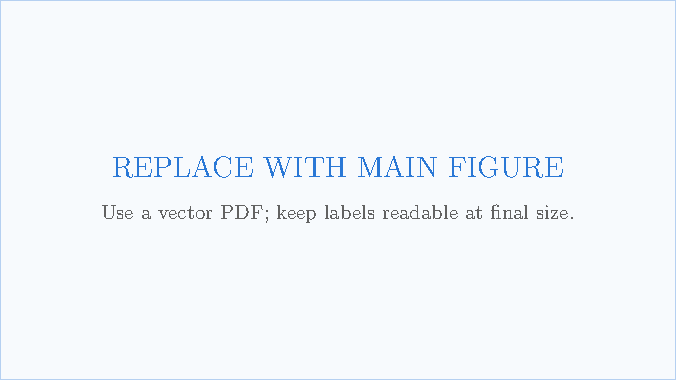
\includegraphics[width=\linewidth,height=.53\textheight,keepaspectratio]{figures/placeholder.pdf}\par
      {\footnotesize\color{Muted}刺激 / 案例说明：\fillin{图中对象、条件与必要来源}}
    \column{.52\textwidth}
      {\color{Accent}任务目标}\par
      \fillin{参与者要做什么；用一句话说明。}\par
      \vspace{.8em}
      {\color{Accent}最少必要规则}\par
      \fillin{只写理解后文所必需的 2–3 条规则。}\par
      \vspace{.8em}
      {\color{Accent}观察到的行为}\par
      \fillin{一次真实输入与输出；不要在这里提前报告模型结果。}
  \end{columns}
  \source{【刺激、任务或案例来源；无来源时写研究设计。】}
\end{frame}

% 04 数据：原始记录长什么样，以及哪些信息需要重建。
\begin{frame}{【原始数据记录什么，又不直接记录什么】}
  \begin{columns}[T,onlytextwidth]
    \column{.56\textwidth}
      \fcolorbox{Accent!25}{Accent!5}{%
        \begin{minipage}[c][3.2cm][c]{.92\linewidth}
          \centering\fillin{放一条去标识化的真实记录、日志或实验事件}
        \end{minipage}}
    \column{.39\textwidth}
      {\color{Accent}直接记录}\par
      \fillin{关键字段与单位。}\par
      \vspace{.7em}
      {\color{Accent}需要重建 / 无法获得}\par
      \fillin{反馈、状态或心理变量的可得性边界。}
  \end{columns}
  \takeaway{【后续预处理为什么必要；只写一个判断。】}
  \source{【数据版本、时间范围与去标识化说明。】}
\end{frame}

% 05 样本：顺序规则与实际删除数，不混用单独命中数。
\begin{frame}{【样本筛选保留了什么分析对象】}
  \vspace{0pt}
  {\small
  \begin{tabular}{@{}r p{4.0cm} p{5.0cm} r@{}}
    \toprule
    & 按顺序执行的规则 & 判定依据 & 实际剩余 \\
    \midrule
    1 & 【规则一】 & 【阈值或操作定义】 & 【数量】 \\
    2 & 【规则二】 & 【阈值或操作定义】 & 【数量】 \\
    3 & 【规则三】 & 【阈值或操作定义】 & 【数量】 \\
    4 & 【最终分析条件】 & 【单位与纳入范围】 & 【数量】 \\
    \bottomrule
  \end{tabular}}
  \takeaway{【最终样本规模与分析单位。】}
  \source{【来源表与口径；“实际删除”与“单独命中”不得混用。】}
\end{frame}

% 06 分析流程：输入 → 处理 / 模型 → 输出。
\begin{frame}{【分析如何把原始行为转成研究证据】}
  \vspace{1.2em}
  \begin{columns}[c,onlytextwidth]
    \column{.27\textwidth}
      \centering\flowbox{输入}{\fillin{原始行为}\par\vspace{.3em}\fillin{已知条件}}
    \column{.06\textwidth}\centering{\color{Accent}\Large $\rightarrow$}
    \column{.36\textwidth}
      \centering\flowbox{处理 / 模型}{\fillin{候选、变量或表征}\par\vspace{.3em}{\small\fillin{主要控制与估计}}}
    \column{.06\textwidth}\centering{\color{Accent}\Large $\rightarrow$}
    \column{.23\textwidth}
      \centering\flowbox{输出}{\fillin{估计或预测}}
  \end{columns}
  \takeaway{【模型输入、比较对象和输出之间最重要的一条关系。】}
\end{frame}

% 07 测量一：定义、公式、例子与核查只保留最关键的一套。
\begin{frame}{【核心测量一的操作定义】}
  \vspace{.8em}
  \begin{columns}[T,onlytextwidth]
    \column{.47\textwidth}
      {\color{Accent}定义}\par
      \fillin{测量对象、方向与单位。}\par
      \vspace{.7em}
      \centering{\Large $\displaystyle \text{【测量一公式】}$}
    \column{.47\textwidth}
      {\color{Accent}一个具体例子}\par
      \fillin{用同一对输入演示数值如何产生。}\par
      \vspace{.7em}
      {\color{Accent}有效性 / 边界}\par
      \fillin{版本、参数和不能解释成什么。}
  \end{columns}
  \source{【测量工具、模型或参数来源。】}
\end{frame}

% 08 测量二：与上一页保持平行结构，便于比较。
\begin{frame}{【核心测量二的操作定义】}
  \vspace{.8em}
  \begin{columns}[T,onlytextwidth]
    \column{.47\textwidth}
      {\color{Accent}定义}\par
      \fillin{测量对象、方向与单位。}\par
      \vspace{.7em}
      \centering{\Large $\displaystyle \text{【测量二公式】}$}
    \column{.47\textwidth}
      {\color{Accent}一个具体例子}\par
      \fillin{用与上一页可比的输入演示。}\par
      \vspace{.7em}
      {\color{Accent}有效性 / 边界}\par
      \fillin{版本、参数和不能解释成什么。}
  \end{columns}
  \source{【测量工具、模型或参数来源；只有一个测量时删除本页。】}
\end{frame}

% 09 模型：公式在上，符号翻译在下；推导放附录。
\begin{frame}{【模型用哪些信息解释或预测结果】}
  \vspace{.5em}
  \centering
  \fcolorbox{Accent!25}{Accent!5}{%
    \begin{minipage}[c][2.0cm][c]{.82\linewidth}
      \centering{\Large $\displaystyle \text{【核心模型公式】}$}
    \end{minipage}}\par
  \vspace{.7em}
  {\small
  \begin{tabular}{@{}l p{8.8cm}@{}}
    \toprule
    符号 & 操作含义 \\
    \midrule
    【符号一】 & 【结果变量或选择对象】 \\
    【符号二】 & 【核心解释变量】 \\
    【符号三】 & 【控制、随机效应或候选集合】 \\
    \bottomrule
  \end{tabular}}
  \takeaway{【估计目标与比较范围。】}
\end{frame}

% 10 评价：对照、样本外验证或稳健性设计在结果前交代。
\begin{frame}{【如何区分新增信息与已有解释】}
  \vspace{.4em}
  {\small
  \begin{tabular}{@{}p{3.2cm} p{5.2cm} p{4.6cm}@{}}
    \toprule
    对照 / 模型 & 相对新增的信息 & 评价口径 \\
    \midrule
    【基线】 & 【已有控制与约束】 & 【系数、误差或预测指标】 \\
    【对照一】 & 【新增测量一】 & 【同一评价口径】 \\
    【对照二】 & 【新增测量二或交互】 & 【同一评价口径】 \\
    \bottomrule
  \end{tabular}}
  \takeaway{【验证按什么单位划分；为什么不会发生信息泄漏。】}
  \source{【拟合、交叉验证、区间估计与排除规则。】}
\end{frame}

% 11–13 三个结果页严格对应第 2 页的三个问题。
% 命令参数：标题、图、横轴、纵轴、点线颜色、take-home、来源。
\fullfigureslide
  {【结果一：回答研究问题一的结论句】}
  {figures/placeholder.pdf}
  {【横轴含义与单位】}
  {【纵轴含义与单位】}
  {【点、线、误差带与颜色分别表示什么】}
  {【唯一 take-home message】}
  {【模型、样本、区间与数据来源】}

\fullfigureslide
  {【结果二：回答研究问题二的结论句】}
  {figures/placeholder.pdf}
  {【横轴含义与单位】}
  {【纵轴含义与单位】}
  {【点、线、误差带与颜色分别表示什么】}
  {【唯一 take-home message】}
  {【模型、样本、区间与数据来源】}

\fullfigureslide
  {【结果三：回答研究问题三的结论句】}
  {figures/placeholder.pdf}
  {【横轴含义与单位】}
  {【纵轴含义与单位】}
  {【点、线、误差带与颜色分别表示什么】}
  {【唯一 take-home message】}
  {【模型、样本、区间与数据来源】}

% 14 边界：只写会改变结论含义的三条边界。
\threepointslide{【结论能够推广到哪里】}
  {【样本边界】}{【纳入与排除如何限制目标总体。】}
  {【测量边界】}{【代理变量或候选集合不能代表什么。】}
  {【推断边界】}{【观察性、预注册状态或外部效度限制。】}

% 15 结论：逐一回答第 2 页，不引入新结果。
\threepointslide{【一句话概括整项研究】}
  {【回答问题一】}{【对应结果一，不复读全部数值。】}
  {【回答问题二】}{【对应结果二，不复读全部数值。】}
  {【回答问题三】}{【对应结果三，说明意义或下一步。】}

% 16 结束页：保留一句核心信息。
\closingslide{谢谢，欢迎讨论}{【一句话核心结论】\par\vspace{.4em}【附录内容或联系方式；可选】}

\appendix
\section{附录}

% 17 附录分隔页。
\sectionslide{A · 附录}{问答所需的补充材料}{操作定义 $\rightarrow$ 数值核查 $\rightarrow$ 补充结果}

% 18 操作定义：正文放不下但必须可核查的口径。
\begin{frame}{附录：【关键变量与参数的操作定义】}
  \normalsize\setlength{\tabcolsep}{3pt}
  \begin{tabular}{@{}p{3.2cm} p{6.0cm} p{4.0cm}@{}}
    \toprule
    项目 & 定义 / 参数 & 来源 \\
    \midrule
    【变量一】 & 【完整定义、方向与单位】 & 【代码 / 文献】 \\
    【变量二】 & 【完整定义、方向与单位】 & 【代码 / 文献】 \\
    【参数一】 & 【固定值与选择依据】 & 【配置 / 文献】 \\
    \bottomrule
  \end{tabular}
  \source{【对应规范文档、提交版本或冻结结果签名。】}
\end{frame}

% 19 数值核查：写覆盖范围，不只写“通过”。
\begin{frame}{附录：【数值与实现核查支持什么】}
  \normalsize\setlength{\tabcolsep}{3pt}
  \begin{tabular}{@{}p{3.0cm} p{6.0cm} p{4.5cm}@{}}
    \toprule
    核查对象 & 方法与独立对照 & 覆盖范围 / 结果 \\
    \midrule
    【样本一致性】 & 【独立重算或跨表核对】 & 【数量与版本】 \\
    【实现正确性】 & 【解析解、单元测试或独立实现】 & 【最大差值】 \\
    【不确定性】 & 【bootstrap、聚类或敏感性拟合】 & 【覆盖范围与限制】 \\
    \bottomrule
  \end{tabular}
  \takeaway{【这些核查能排除什么，不能排除什么。】}
\end{frame}

% 20 补充结果：仍使用与正文完全相同的图注和 take-home 结构。
\fullfigureslide
  {附录：【补充结果的有限结论】}
  {figures/placeholder.pdf}
  {【横轴含义与单位】}
  {【纵轴含义与单位】}
  {【点、线、误差带与颜色分别表示什么】}
  {【补充结果改变了什么，或没有改变什么】}
  {【模型、样本、区间与数据来源】}

\end{document}
